\documentclass{article}
\usepackage{listings}
\usepackage{graphicx}
\usepackage[left=6em, right=2cm, top=1cm,bottom=1.75cm]{geometry}

\lstset{
	language=c++,
	breaklines=true,
	showstringspaces=false
	}

\begin{document}
\tableofcontents
\addtocontents{toc}{~\hfill\textbf{Page}\par}
\thispagestyle{empty}
\newpage
\setcounter{page}{1}
\begin{flushleft}
\section {To implement 3x3 sparse matrix.}

\begin{lstlisting}
#include<bits/stdc++.h>
using namespace std;
#define ll long long
#define loop(i,a,b) for(ll i=a;i<b;i++)
int main()
{
ll A[3][3]={0};
ll n,x,y,v;
 cin>>n;
 loop(i,0,n)
 {
cin>>x>>y>>v;
 A[x][y]=v;
 }
 loop(i,0,3)
 { loop(j,0,3)
   cout<<A[i][j]<<" ";
 cout<<endl;
}
}

\end{lstlisting}

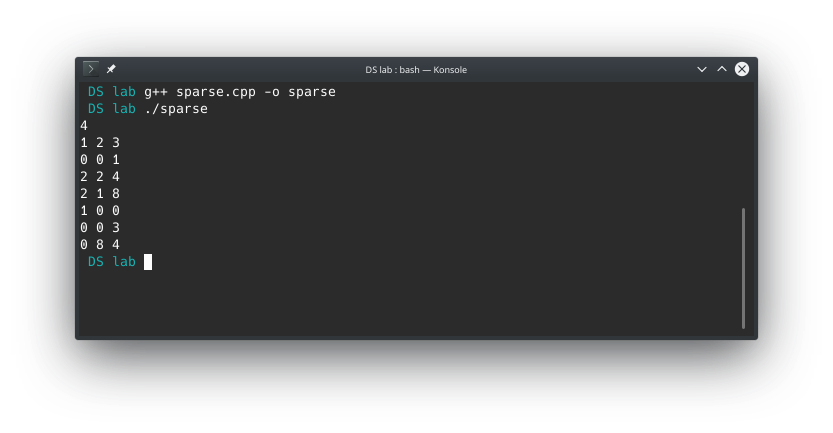
\includegraphics[width=\linewidth]{1.png}
\pagebreak
\section {To implement rxc sparse matrix.}

\begin{lstlisting}
#include<bits/stdc++.h>
using namespace std;
#define ll long long
#define loop(i,a,b) for(ll i=a;i<b;i++)
int main()
{
ll n,x,y,v;
ll r,c;
cin>>r>>c;

ll A[r][c];
memset(A,0,sizeof(A));
 cin>>n;
 loop(i,0,n)
 {
cin>>x>>y>>v;
 A[x][y]=v;
 }
 loop(i,0,r)
 { loop(j,0,c)
   cout<<A[i][j]<<" ";
 cout<<endl;
}
}

\end{lstlisting}

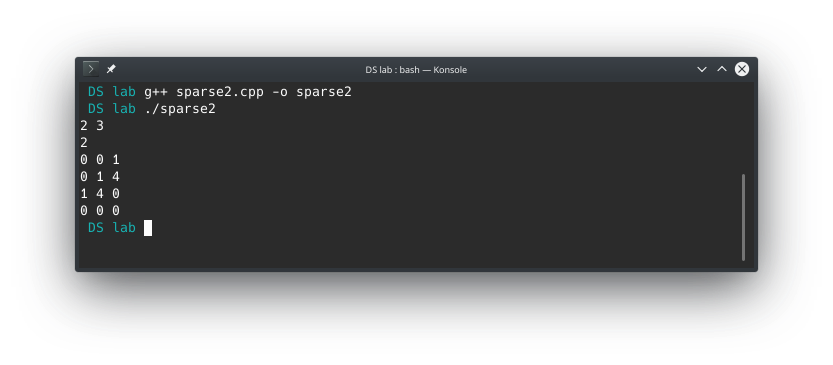
\includegraphics[width=\linewidth]{2.png}
\pagebreak
\section{Write a program to implement linear search.}
\begin{lstlisting}
#include<bits/stdc++.h>
using namespace std;
#define ll long long
#define loop(i,a,b) for(ll i=a;i<b;i++)
int main()
{
ll n,x,f=0;
	cin>>n;
 cin>>x;
ll A[n];
 loop(i,0,n)
  cin>>A[i];
 loop(i,0,n)
  if(A[i]==x)
   {
 f=1;
break;
}
if(f) cout<<"FOUND";
else cout<<"NOT FOUND\n";
}

\end{lstlisting}

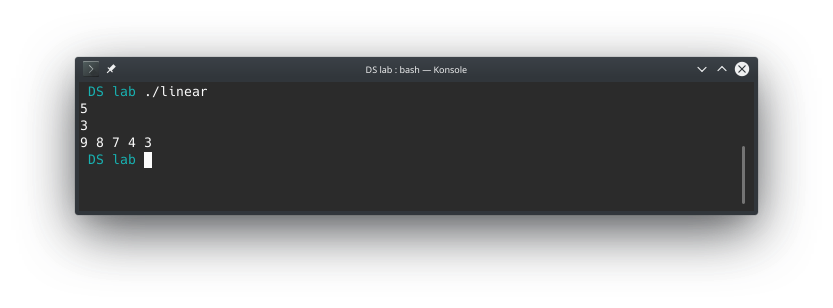
\includegraphics[width=\linewidth]{3.png}
\pagebreak
\section{Write a program to implement binary search.}
\begin{lstlisting}
#include<bits/stdc++.h>

using namespace std;
#define ll long long
#define loop(i,a,b) for(ll i=a;i<b;i++)
int main()
{



	ll n,x,l,u,f=0;
	cin>>n;
ll A[n];
	loop(i,0,n)
  	 cin>>A[i];
	cin>>x;
	l=0;
	u=n-1;
	while(l<=u)
	{
 	 ll m=(u+l)>>1;
 	 if(A[m]>x)
          u=m-1;
	 else if(A[m]<x)
	  l=m+1;
	 else
	 { f=1;break;}
	}
	if(f) cout<<"FOUND\n";
	else cout<<"NOT FOUND\n";

}

\end{lstlisting}

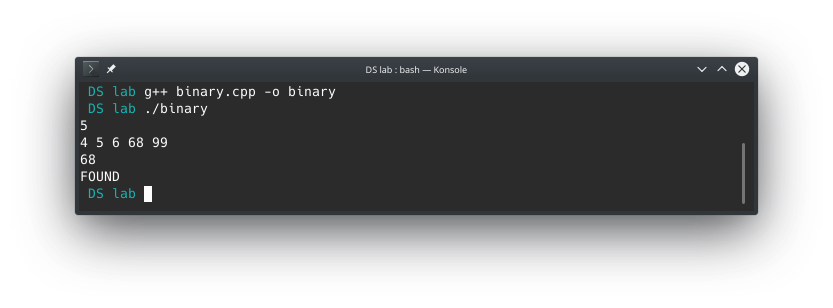
\includegraphics[width=\linewidth]{4.png}

\pagebreak
\section{Write a program to implement following operation in stack.}
\subsection{To push element into stack.}
\subsection{To pop from stack.}
\subsection{To print top element.}
\begin{lstlisting}
#include<bits/stdc++.h>
using namespace std;
int A[1000],top=-1,size;
void push()
{
    if(top==size-1)
	cout<<"Stack is full\n";
    else
    {
	  int n;
	  cout<<"Enter the element. ";
	  cin>>n;
	  A[++top]=n;
	  cout<<"Element is successfully added\n";
    }
}
void pop()
{
    if(top==-1)
	cout<<"Stack is empty\n";
    else
	cout<<A[top--]<<" is poped\n";
}
void peek()
{
    if(top==-1)
	cout<<"Stack is empty\n";
    else
	cout<<A[top]<<" is at top\n";
}
int main()
{
    char ch;
    cout<<"ENter the size of stack. ";
    cin>>size;
    do
    {
	int c;
	cout<<"Enter \n\t1. To Push\n\t2. To Pop\n\t 3. To find top element ";
	cin>>c;
	switch(c)
	  {
	      case 1: {
		  push();
	      }
	      break;
	      case 2: pop();
	      break;
	      case 3:peek();
	  }

	  for(int i=top;i>=0;i--)
	      cout<<A[i]<<endl;
	  cout<<"Do you want to continue? ";
	  cin>>ch;
    }while(ch=='y');
}

\end{lstlisting}

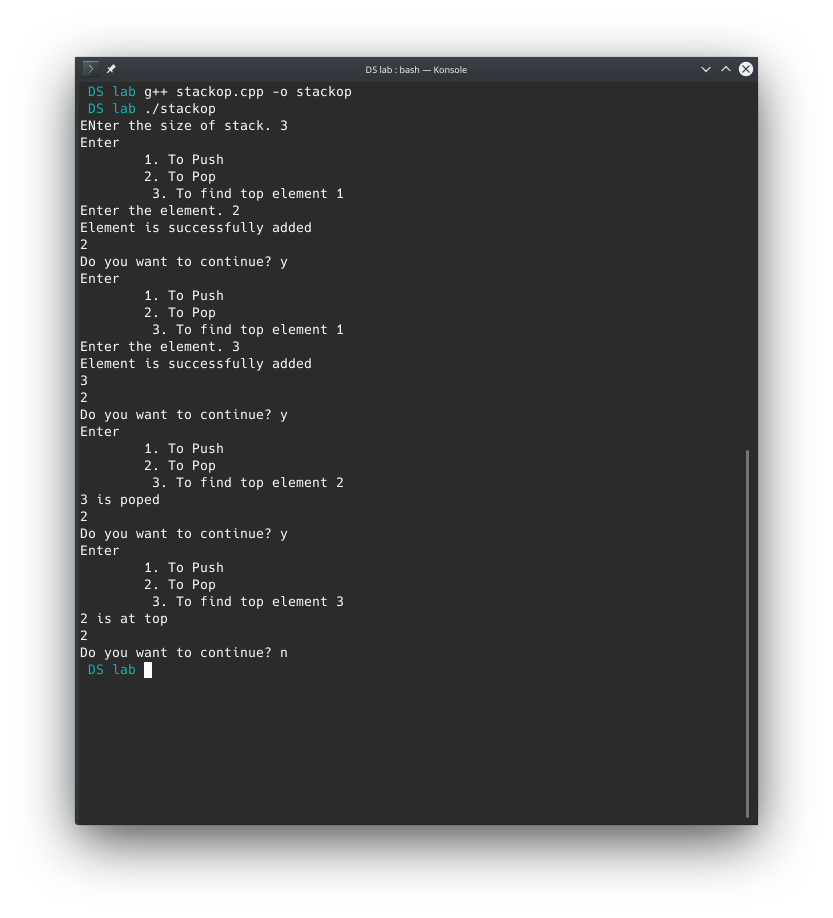
\includegraphics[width=\linewidth]{5.png}

\pagebreak
\section{Write a program to find the reverse of the string using stack.}
\begin{lstlisting}
#include<bits/stdc++.h>
using namespace std;
char A[1000];int top=-1,size;
void push()
{
    if(top==size-1)
	cout<<"Stack is full\n";
    else
    {
	 char c;
	  cin>>c;
	  A[++top]=c;
    }
}
void pop()
{
    if(top==-1)
	cout<<"Stack is empty\n";
    else
	cout<<A[top--];
}
int main()
{

	cout<<"enter size and string\n";
	cin>>size;
	for(int i=0;i<size;i++)
	    push();
	for(int i=0;i<size;i++)
	    pop();
    cout<<endl;
}

\end{lstlisting}

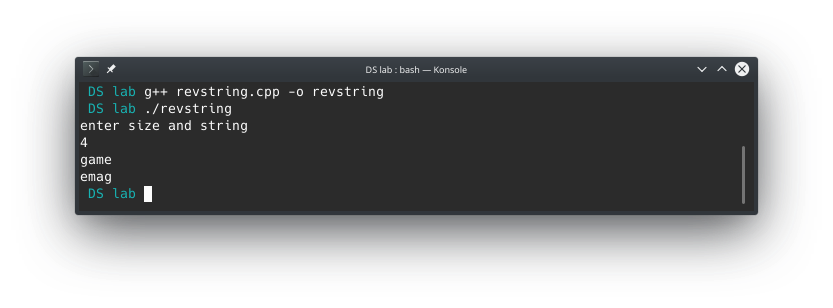
\includegraphics[width=\linewidth]{6.png}

\pagebreak
\section{Write a program to find whether a string is palindrome or not.}
\begin{lstlisting}
#include<bits/stdc++.h>
using namespace std;
char A[1000];int top=-1,size;
void push(char c)
{
    if(top==size-1)
	cout<<"Stack is full\n";
    else
    {
	  A[++top]=c;
    }
}
char pop()
{
    if(top==-1)
	cout<<"Stack is empty\n";
    else
    return A[top--];
}
int main()
{

	cout<<"enter size and string\n";
	cin>>size;
	char s[size],a[size];
	cin>>s;
	for(int i=0;i<size;i++)
	    push(s[i]);
	for(int i=0;i<size;i++)
	    a[i]=pop();
	if(strcmp(a,s)==0)
	    cout<<"Palandrom";
	else cout<<"NoT palandrom";
}

\end{lstlisting}


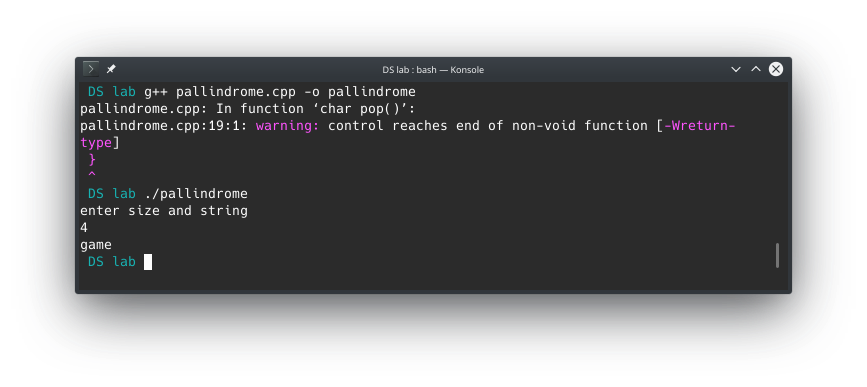
\includegraphics[width=\linewidth]{7.png}
\pagebreak
\section{Write a program to implement queue using array.}
\begin{lstlisting}

#include<bits/stdc++.h>
using namespace std;

#define ll long
ll A[100],front=-1,n,rear=-1;
void insert()
{
    if(rear==n-1)
	cout<<"Overflow";
    else
    {
	cout<<"Enter element you want to enter";
	ll x;
	cin>>x;
	A[++rear]=x;
    }
}

void dlete()
{
    if(front>=rear)
	cout<<"Underflow\n";
    else
    {
	cout<<A[++front]<<" Deleted";
    }
}

void frnt()
{
    if(front>=rear)
	cout<<"Underflow\n";
    else
    {
	cout<<A[front+1]<<" is at fornt";
    }
}

int main()
{
    ll c;
    char ch;
    cout<<"Enter size of array";
    cin>>n;
    do{
	cout<<"Enter \n\t1.To insert\n\t2.To delete\n\t3.To  front";
	cin>>c;
	switch(c)
	{
	    case 1: insert();
	    break;
	    case 2: dlete();
	    break;
	    case 3: frnt();
	}
	cout<<"queue is ";
	for(ll i=front+1;i<=rear;i++)
	     cout<<A[i]<<" ";
	    cout<<endl;
	cout<<"Do you want to continue?";
	cin>>ch;
    }while(ch=='y');
}


\end{lstlisting}

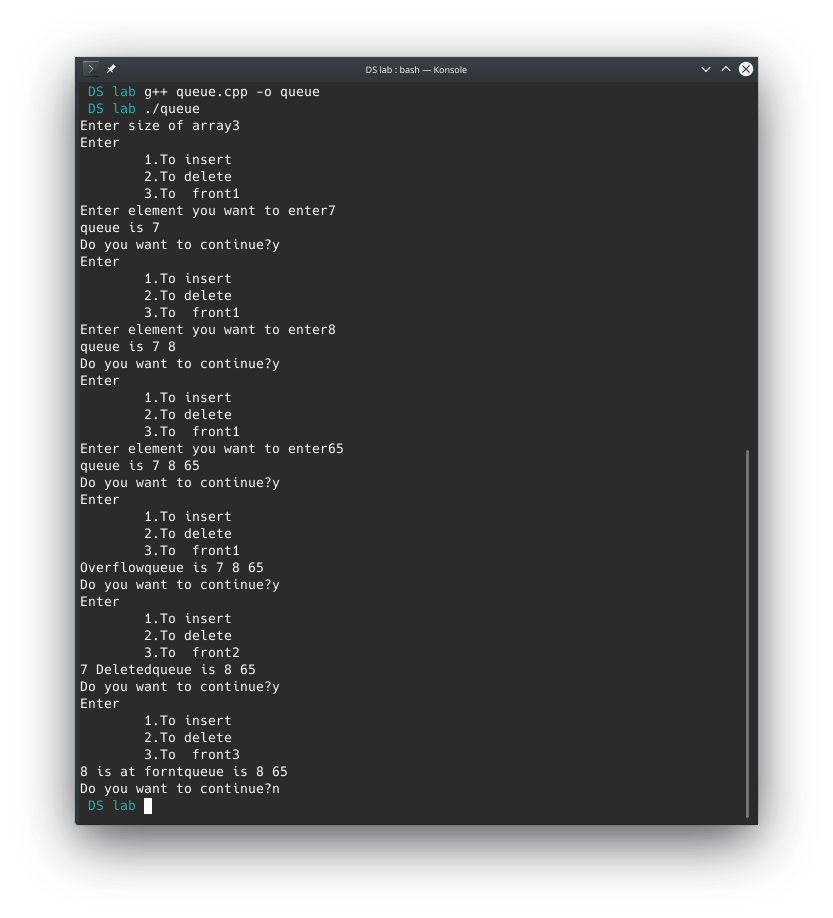
\includegraphics[width=\linewidth]{8.png}

\pagebreak
\section{Write a program to implement a circular queue using an array.}
\begin{lstlisting}

#include<bits/stdc++.h>
using namespace std;

#define ll long
ll A[100],front=-1,n,rear=-1;
void insert()
{
    if((rear==n-1 && front==0) || (rear+1==front ))
	cout<<"Overflow \n";

    else
    {
	cout<<"Enter element you want to enter";
	ll x;
	cin>>x;
	rear=(rear+1)%n;
	A[rear]=x;
	if(front==-1)
	    front=0;
    }
}

void dlete()
{
    if(front==rear&& rear==-1)
	cout<<"Underflow\n";
    else
    {
	cout<<A[front]<<" Deleted";
	if(front==rear)
	    rear=front=-1;
	else
		front=(front+1)%n;
    }
}

void frnt()
{
    if(front==rear&& rear==-1)
	cout<<"Underflow\n";
    else
    {
	cout<<A[front]<<" is at fornt";
    }
}

int main()
{
    ll c;
    char ch;
    cout<<"Enter size of array";
    cin>>n;
    do{
	cout<<"Enter \n\t1.To insert\n\t2.To delete\n\t3.To  front";
	cin>>c;
	switch(c)
	{
	    case 1: insert();
	    break;
	    case 2: dlete();
	    break;
	    case 3: frnt();
	}
	cout<<"Do you want to continue?";
	cin>>ch;
    }while(ch=='y');
}


\end{lstlisting}

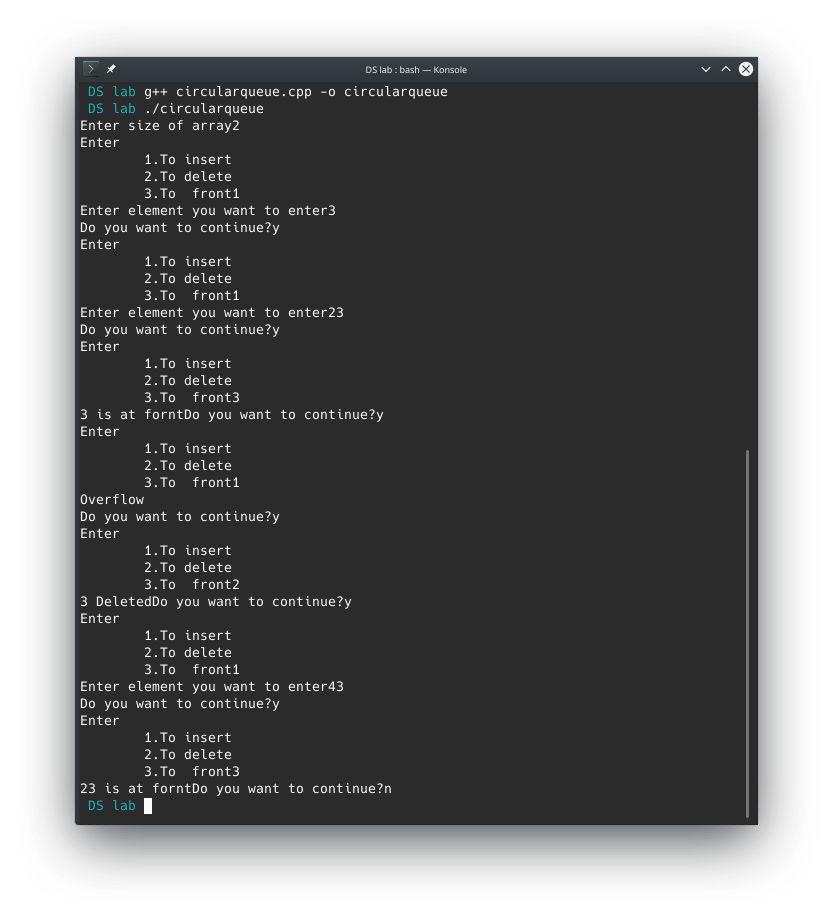
\includegraphics[width=\linewidth]{9.png}
\pagebreak
\section{Write a program to convert infix to postfix.}
\begin{lstlisting}
#include<bits/stdc++.h>
using namespace std;
#define ll long long
#define loop(i,a,b) for(ll i=a;i<b;i++)

#define pb push_back
ll check(char c)
{
    if(c=='*' || c=='/')
	return 2;
    else
	return 1;
}
int main()
{
    string s;
    stack<char> op;
    string ans;
    cin>>s;
    loop(i,0,s.length())
    {
	if(s[i]=='+' || s[i]=='-' || s[i]=='*' || s[i]=='/' )
	{
	    while(!op.empty() && (check(op.top())>check(s[i])))
	    {
		ans.pb(op.top());
		op.pop();
		if(op.empty())
		    break;
	    }
	    op.push(s[i]);
 	 }

	else if(s[i]=='(')
	    op.push(s[i]);
	else if(s[i]==')')
	{
	    while(!op.empty() && op.top()!='('){
	     ans.pb(op.top());
	     op.pop();
	    }
	    op.pop();
	}
	else
	    ans.pb(s[i]);

    }
    while(!op.empty()){
	ans.pb(op.top());
	op.pop();
    }
    cout<<ans<<endl;
}


\end{lstlisting}

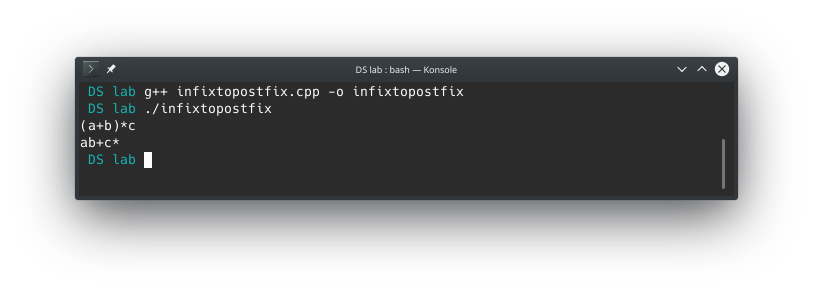
\includegraphics[width=\linewidth]{10.png}

\pagebreak
\section{Write a program to implement priority queue.}
\lstinputlisting{test.cpp}
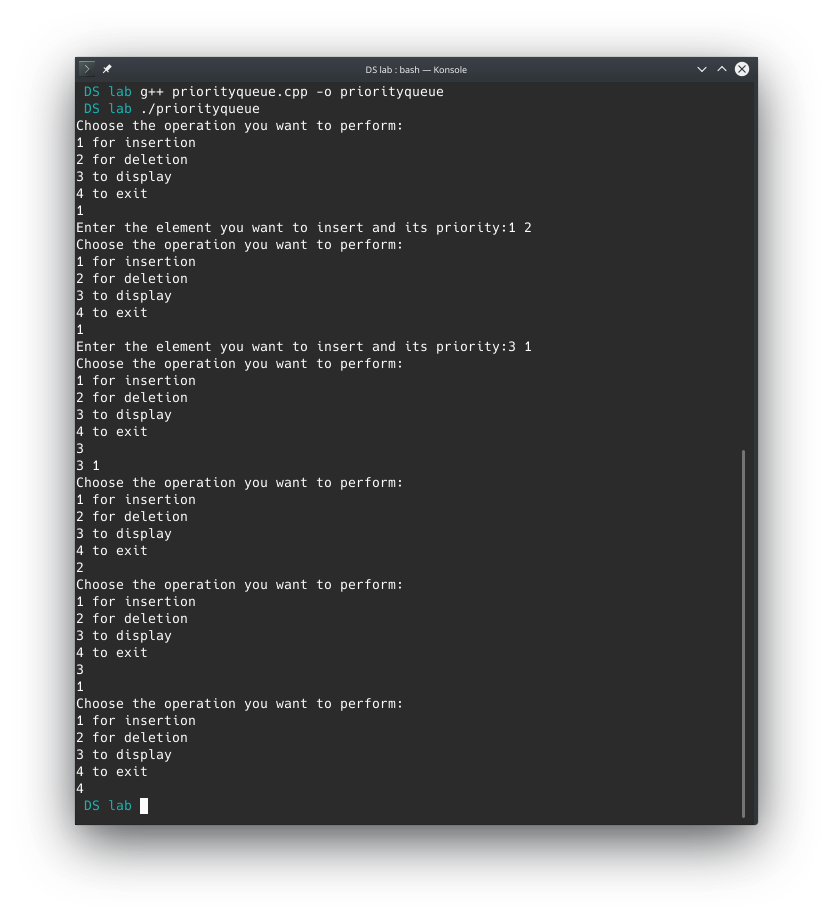
\includegraphics[width=\linewidth]{11.png}
\pagebreak
\section{Given two integers n and m, in a single operation n can be multiplied by either 2 or 3. Write a program to find the minimum number of given operati to convert n into m. If it is impossible to convert n to m with the given operation then print -1.}
\begin{lstlisting}
#include<stdio.h>

int main()
{
	int n,m,flag=1,c2=0,c3=0;
	double n1,m1;

	scanf("%d %d",&n,&m);

	n1 = n;
	m1 = m;

	m1/=n1;
	m/=n;

	if(m<m1)
	{
		printf("-1 \n");
		return 0;
	}

	while(flag)
	{
		flag = 0;

		if(m%2==0)
		{
			m/=2;
			c2++;
			flag = 1;
		}
		else if(m%3==0)
		{
			m/=3;
			c3++;
			flag = 1;
		}
		else if(m==1)
		{
			printf("%d \n",c2+c3);
			return 0;
		}
	}

	printf("-1 \n");

	return 0;
}

\end{lstlisting}

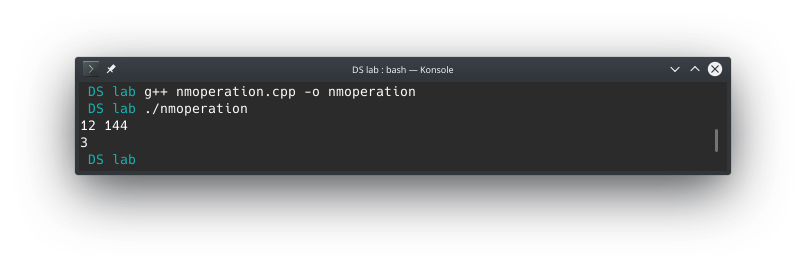
\includegraphics[width=\linewidth]{12.png}

\pagebreak
\section{Write a program to implement following operation.}
\subsection{To insert an element in linked list.}
\subsection{To delete an element from linked list.}
\subsection{To traverse }
\begin{lstlisting}
#include<bits/stdc++.h>
using namespace std;

#define ll long long
#define loop(i,a,b) for(ll i=a;i<b;i++)

struct node
{
    int data;
    node *next;
}*head=NULL;

void inser()
{
    ll x,n;
    cout<<"\nEnter the value and its position ";
    cin>>x>>n;
    node* temp= new node;
    node* temp1=new node;
    temp1->data=x;
    temp1->next=NULL;
    temp=head;
    ll j=temp1->data;
    if(n==1){
	temp1->next=head;
	head=temp1;
    }
    else{
    ll c=1;
    while(c!=n-1 && temp->next!=NULL){
	c++;
	temp=temp->next;
    }
	temp1->next=temp->next;
	temp->next=temp1;
     j=temp->data;
     ll k=temp1->data;
     ll n=head->data;
    }
     j=head->data;
    cout<<head->data;
}
void delet()
{
    cout<<"\nEnter position u wamt to delete\n";
    ll x;
    cin>>x;
    x--;
    node *temp=new node;
    temp=head;
    while(--x && temp!=NULL)
	temp=temp->next;
	if(head==NULL || x!=0)
	    cout<<"Ma chuda\nbhuddi khol ke input do\n";
	else{

    temp->next=temp->next->next;
	}
}

void traverse()
{
    node *temp=new node;
    cout<<"Linked list is \n";

    temp=head;
    ll j=head->data;
    ll k=temp->data;
    while(temp!=NULL)
	{
	    cout<<temp->data<<" ";
	    temp=temp->next;
	}
}



int main()
{

   ll ch;
   do{
       cout<<"Enter 1.To Insertion \n\t2.To delete \n\t3.To traverse\n\t4.To exit ";
       cin>>ch;

       switch(ch)
       {
	   case 1:
	    inser();
	    break;
	   case 2:
	    delet();
	    break;
	   case 3:
	    traverse();
	}


	}while(ch!=4);

}

\end{lstlisting}
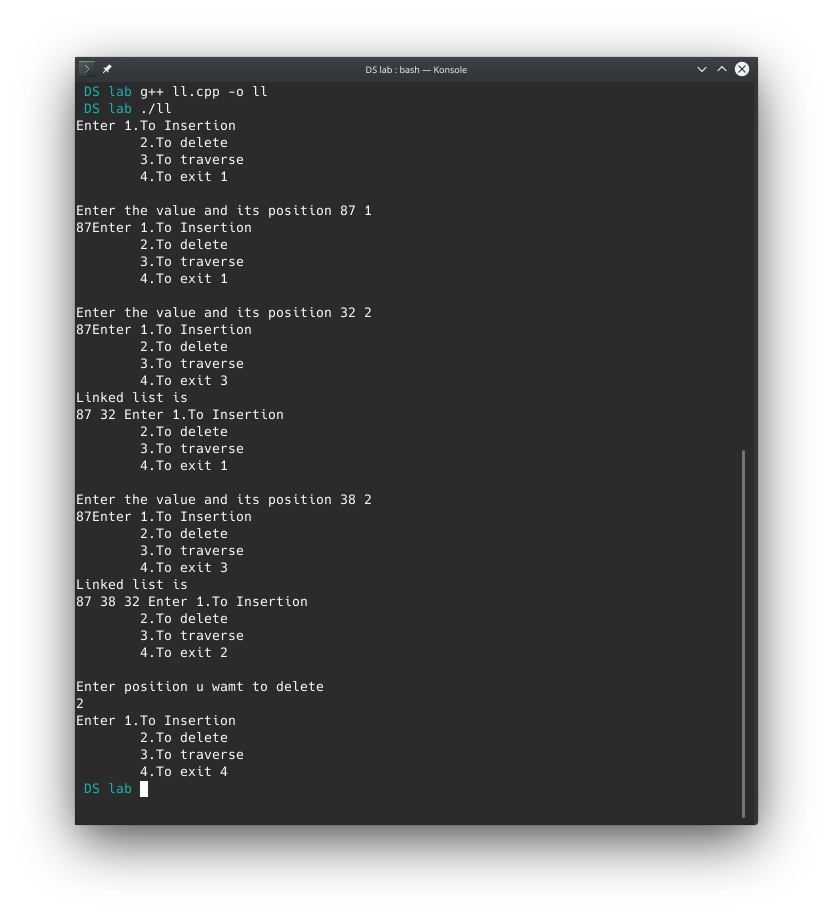
\includegraphics[width=\linewidth]{13.png}


\pagebreak
\section{Given a Linked List of integers, write a program to print the linked list such that all even numbers appear before all the odd numbers in the linked list. Also, keep the order of even and odd numbers same.}
\begin{lstlisting}
#include<bits/stdc++.h>
using namespace std;

#define ll long long
#define loop(i,a,b) for(ll i=a;i<b;i++)

struct node
{
    int data;
    node *next;
}*head=NULL;

void inser()
{
    ll x,n;
    cout<<"\nEnter the value and its position ";
    cin>>x>>n;
    node* temp= new node;
    node* temp1=new node;
    temp1->data=x;
    temp1->next=NULL;
    temp=head;
    ll j=temp1->data;
    if(n==1){
	temp1->next=head;
	head=temp1;
    }
    else{
    ll c=1;
    while(c!=n-1 && temp->next!=NULL){
	c++;
	temp=temp->next;
    }
	temp1->next=temp->next;
	temp->next=temp1;
     j=temp->data;
     ll k=temp1->data;
     ll n=head->data;
    }
     j=head->data;
}
void delet()
{
    cout<<"\nEnter position u wamt to delete\n";
    ll x;
    cin>>x;
    x--;
    node *temp=new node;
    temp=head;
    while(--x && temp!=NULL)
	temp=temp->next; 
	if(head==NULL || x!=0)
	    cout<<"Ma chuda\nbhuddi khol ke input do\n";
	else{
	    
    temp->next=temp->next->next;
	}
}

void traverse()
{
    node *temp=new node;
    cout<<"Linked list is \n";

    temp=head;
    ll j=head->data;
    ll k=temp->data;
    while(temp!=NULL)
	{
	    cout<<temp->data<<" ";
	    temp=temp->next;
	}
}



void op()
{
    node *temp=new node;
    cout<<"After operation list is \n";
    vector<ll> O,E;

    temp=head;
    ll j=head->data;
    ll k=temp->data;
    ll c=0;
    while(temp!=NULL)
	{
	    c++;
	    if(c%2)
		O.push_back(temp->data);
	    else
		E.push_back(temp->data);

	    temp=temp->next;
	}
	loop(i,0,O.size())
	 cout<<O[i]<<" -> ";
	loop(i,0,E.size())
	 cout<<E[E.size()-i-1]<<" -> ";
	cout<<"NULL\n";

}



int main()
{
   
   ll ch;
   do{
       cout<<"\nEnter 1.To Insertion \n\t2.To delete \n\t3.To traverse\n\t4.To operation \n\t5.To exit ";
       cin>>ch;
       
       switch(ch)
       {
	   case 1:
	    inser();
	    break;
	   case 2:
	    delet();
	    break;
	   case 3:
	    traverse();
	    break;
	   case 4: op();
	}


	}while(ch!=5);

}

\end{lstlisting}


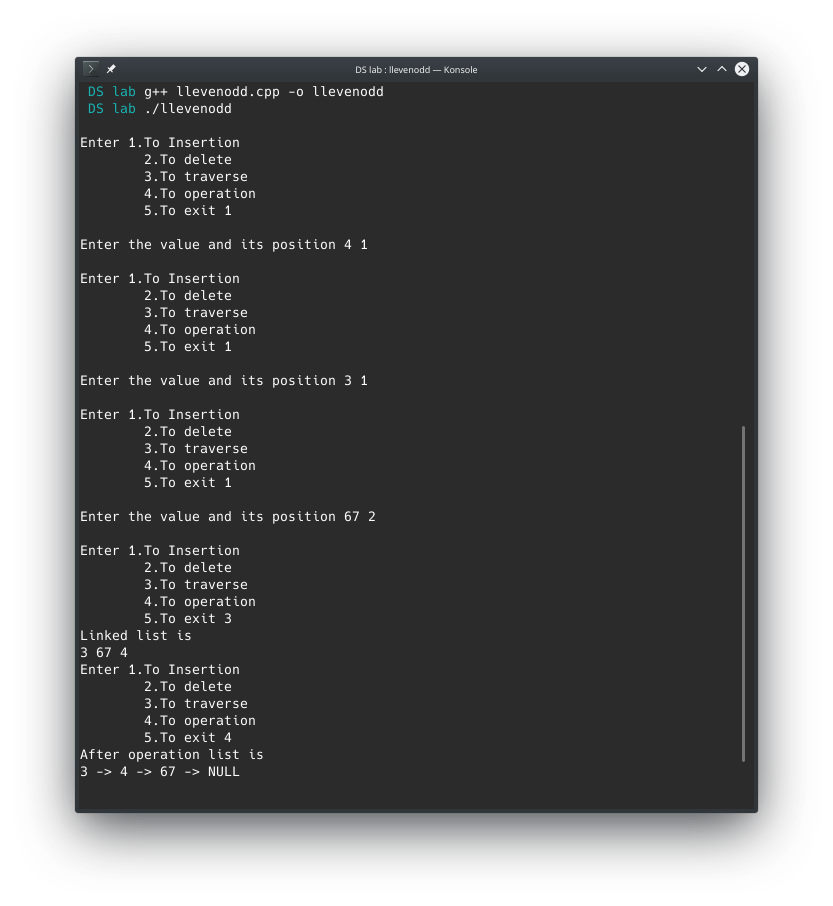
\includegraphics[width=\linewidth]{14.png}

\pagebreak
\section{Write a program to perform following operation on doubly linked list.}
\subsection{To add an element at head.}
\subsection{To add an element after a node.}
\subsection{To add an element at tail.}
\subsection{To add an element before a node.}
\begin{lstlisting}
#include<bits/stdc++.h>
using namespace std;

#define ll long long
#define loop(i,a,b) for(ll i=a;i<b;i++)
ll c=0;

struct node{
    ll val;
    node * next;
    node * prev;
}*head=NULL;
void insert(ll y,ll x)
{

    node *temp=new node;
    temp->val=x;
    temp->next=NULL;
    temp->prev=NULL;
    if(head==NULL){
	if(y==0)
	    head=temp,c++;
	else
	    cout<"dimag to sahi hai ";
    }
    else
    {
	if(y==0)
	{
	    c++;
	    node *temp1=head;
	    temp1->prev=temp;
	    head=temp;
	    head->next=temp1;
	    return ;
	}
	ll co=0;
	ll f=0;
	node * temp1=head;
	while(temp1!=NULL)
	{
	    co++;
	    if(y==co){
		f=1;
		break;
	    }
	    temp1=temp1->next;
	}
	if(f)
	{
	    c++;
	    temp->next=temp1->next;
	    if(temp1->next!=NULL)
	    temp1->next->prev=temp;
	    temp1->next=temp;
	    temp->prev=temp1;
	}
	else
	     cout<<"Dimag to sahi hai "<<endl;
    }
}
	    

	
void disp()
{
    node *temp=head;
    cout<<"\n Doubly linked list have element\n";
    while(temp!=NULL)
    {
	cout<<temp->val<<" ";
	temp=temp->next;
    }
    cout<<endl;
}



int main()
{
    ll ch,x,y;
    do{
	cout<<"Enter \n\t1.To enter at the front.\n\t2.To add after a given node\n\t3.Add a node at the last.\n\t4.Add a node before a given node\n\t5.Exit. ";
	cin>>ch;
	switch(ch){
	    case 1:
	     cout<<"Enter value of the node";
	     cin>>x;
	     insert(0,x);
	     break;
	    case 2:
	     cout<<"Enter value of the node and position of node after which it is going to store ";
	     cin>>x>>y;
	     insert(y,x);
	     break;
	    case 3:
	     cout<<"Enter value of the node";
	     cin>>x;
	     insert(c,x);
	     break;
	    case 4:
	     cout<<"Enter value of the node and position of node before which it is going to stoe ";
	     cin>>x>>y;
	     insert(y-1,x);
	     break;
	}
	if(c)
	disp();
    }while(ch!=5);
}

\end{lstlisting}


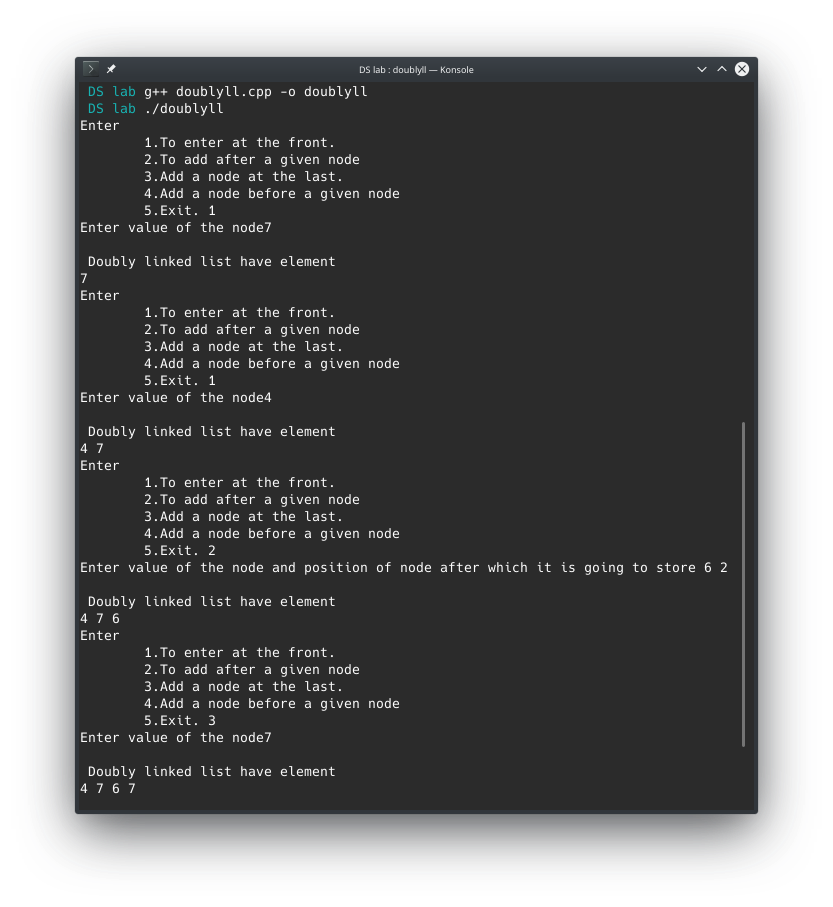
\includegraphics[width=\linewidth]{15.png}

\pagebreak
\section{Given a doubly linked list containing N nodes. The task is to find the product of all prime nodes.}
\begin{lstlisting}
#include<bits/stdc++.h>
using namespace std;

#define ll long long
#define loop(i,a,b) for(ll i=a;i<b;i++)
ll c=0;

struct node{
    ll val;
    node * next;
    node * prev;
}*head=NULL;
void insert(ll y,ll x)
{

    node *temp=new node;
    temp->val=x;
    temp->next=NULL;
    temp->prev=NULL;
    if(head==NULL){
	if(y==0)
	    head=temp,c++;
	else
	    cout<"dimag to sahi hai ";
    }
    else
    {
	if(y==0)
	{
	    c++;
	    node *temp1=head;
	    temp1->prev=temp;
	    head=temp;
	    head->next=temp1;
	    return ;
	}
	ll co=0;
	ll f=0;
	node * temp1=head;
	while(temp1!=NULL)
	{
	    co++;
	    if(y==co){
		f=1;
		break;
	    }
	    temp1=temp1->next;
	}
	if(f)
	{
	    c++;
	    temp->next=temp1->next;
	    if(temp1->next!=NULL)
	    temp1->next->prev=temp;
	    temp1->next=temp;
	    temp->prev=temp1;
	}
	else
	     cout<<"Dimag to sahi hai "<<endl;
    }
}


ll A[10000]={0};

void func()
{
    ll f=1,ans=1;
    node *temp=head;
    while(temp!=NULL)
    {
	if(A[temp->val]==0){
	    f=1;
	    ans*=temp->val;
	}
	temp=temp->next;
    }
    if(f)
    cout<<"\nproduct is "<<ans;
    else cout<<"No prime no \n";
}


void disp()
{
    node *temp=head;
    cout<<"\n Doubly linked list have element\n";
    while(temp!=NULL)
    {
	cout<<temp->val<<" ";
	temp=temp->next;
    }
    cout<<endl;
}



int main()
{
    for(ll i=2;i*i<=10000;i++)
	if(A[i]==0)
	for(ll j=2*i;j<=10000;j+=i)
    		A[j]=1;

    ll ch,x,y;
    do{
	cout<<"\nEnter \n\t1.To enter at the front.\n\t2.To add after a given node\n\t3.Add a node at the last.\n\t4.Add a node before a given node\n\t5.To operation \n\t6.Exit. ";
	cin>>ch;
	switch(ch){
	    case 1:
	     cout<<"Enter value of the node";
	     cin>>x;
	     insert(0,x);
	     break;
	    case 2:
	     cout<<"Enter value of the node and position of node after which it is going to store ";
	     cin>>x>>y;
	     insert(y,x);
	     break;
	    case 3:
	     cout<<"Enter value of the node";
	     cin>>x;
	     insert(c,x);
	     break;
	    case 4:
	     cout<<"Enter value of the node and position of node before which it is going to store ";
	     cin>>x>>y;
	     insert(y-1,x);
	     break;
	    case 5: func();
	}
	if(c && ch!=5)
	disp();
    }while(ch!=6);
}

\end{lstlisting}

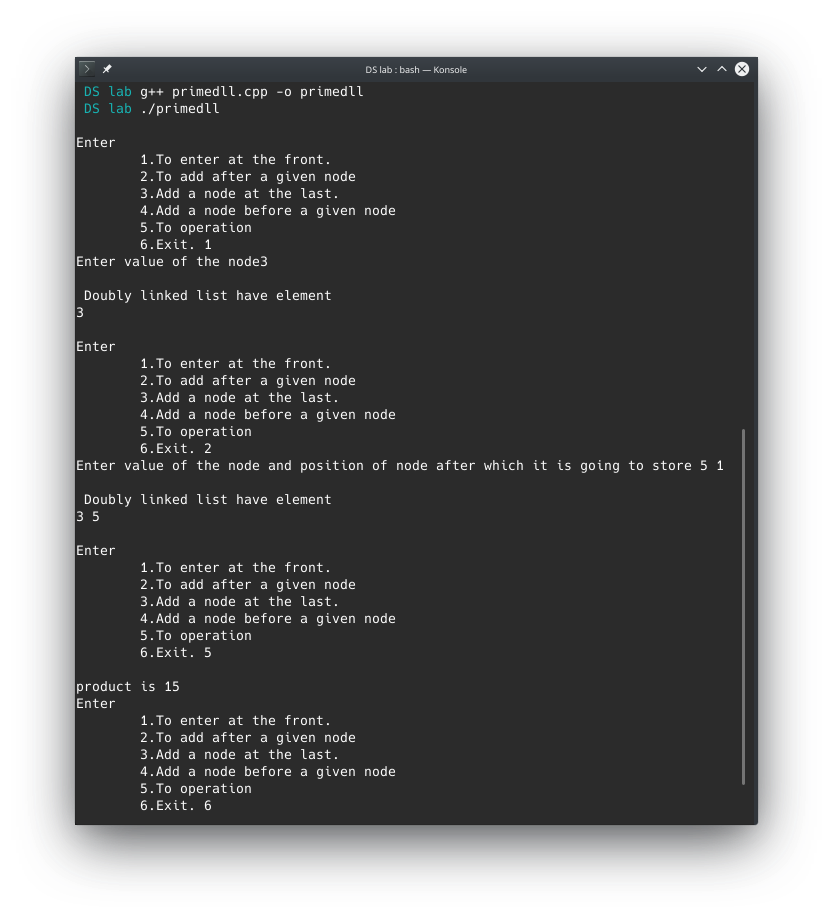
\includegraphics[width=\linewidth]{16.png}


\pagebreak
\section{Given a sorted doubly linked list of positive distinct elements, write a program to find pairs in the doubly linked list whose product is equal to given value x, without using any extra space.}
\begin{lstlisting}
#include<bits/stdc++.h>
using namespace std;

#define ll long long
#define loop(i,a,b) for(ll i=a;i<b;i++)
ll c=0;

struct node{
    ll val;
    node * next;
    node * prev;
}*head=NULL;
void insert(ll y,ll x)
{

    node *temp=new node;
    temp->val=x;
    temp->next=NULL;
    temp->prev=NULL;
    if(head==NULL){
	if(y==0)
	    head=temp,c++;
	else
	    cout<"dimag to sahi hai ";
    }
    else
    {
	if(y==0)
	{
	    c++;
	    node *temp1=head;
	    temp1->prev=temp;
	    head=temp;
	    head->next=temp1;
	    return ;
	}
	ll co=0;
	ll f=0;
	node * temp1=head;
	while(temp1!=NULL)
	{
	    co++;
	    if(y==co){
		f=1;
		break;
	    }
	    temp1=temp1->next;
	}
	if(f)
	{
	    c++;
	    temp->next=temp1->next;
	    if(temp1->next!=NULL)
	    temp1->next->prev=temp;
	    temp1->next=temp;
	    temp->prev=temp1;
	}
	else
	     cout<<"Dimag to sahi hai "<<endl;
    }
}



void func()
{
	node * temp1,*temp2;
	temp1=head;
	ll x;
	cout<<"Enter x ";
	cin>>x;
	while(temp1!=NULL)
	{
	    temp2=head;
	    while(temp2!=NULL)
	    {
		if(temp1->val*temp2->val==x)
		    cout<<"("<<temp1->val<<","<<temp2->val<<")\n";
		   temp2=temp2->next;
	    }

		   temp1=temp1->next;
	}
}


void disp()
{
    node *temp=head;
    cout<<"\n Doubly linked list have element\n";
    while(temp!=NULL)
    {
	cout<<temp->val<<" ";
	temp=temp->next;
    }
    cout<<endl;
}



int main()
{

    ll ch,x,y;
    do{
	cout<<"\nEnter \n\t1.To enter at the front.\n\t2.To add after a given node\n\t3.Add a node at the last.\n\t4.Add a node before a given node\n\t5.To operation \n\t6.Exit. ";
	cin>>ch;
	switch(ch){
	    case 1:
	     cout<<"Enter value of the node";
	     cin>>x;
	     insert(0,x);
	     break;
	    case 2:
	     cout<<"Enter value of the node and position of node after which it is going to store ";
	     cin>>x>>y;
	     insert(y,x);
	     break;
	    case 3:
	     cout<<"Enter value of the node";
	     cin>>x;
	     insert(c,x);
	     break;
	    case 4:
	     cout<<"Enter value of the node and position of node before which it is going to stoe ";
	     cin>>x>>y;
	     insert(y-1,x);
	     break;
	    case 5: func();
	}
	if(c && ch!=5)
	disp();
    }while(ch!=6);
}

\end{lstlisting}

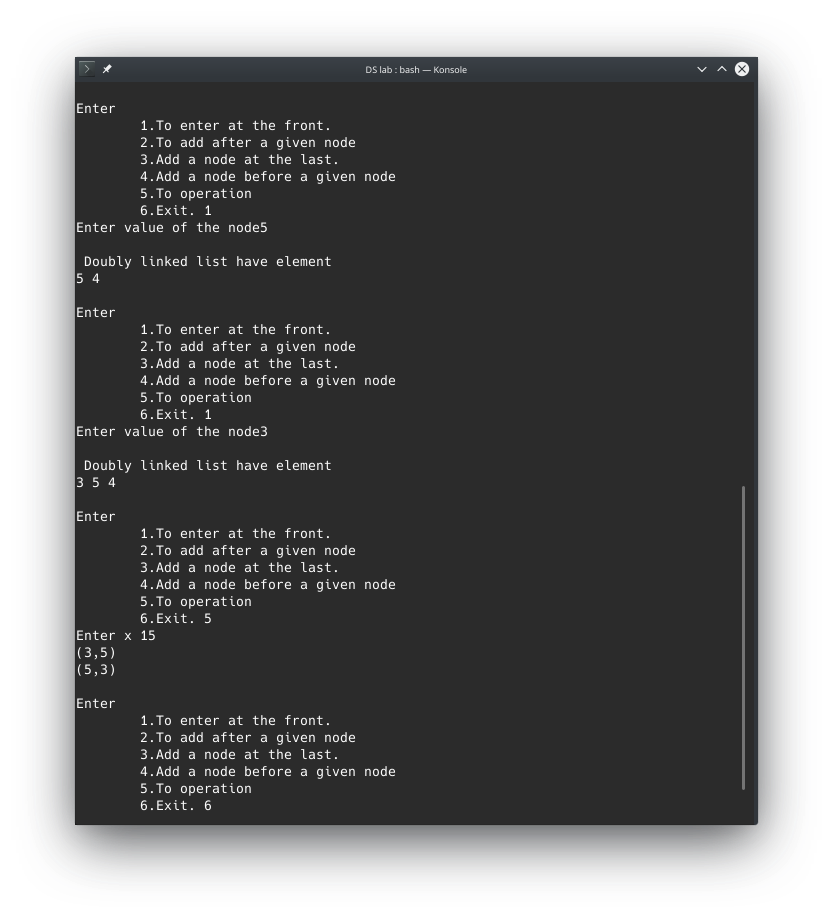
\includegraphics[width=\linewidth]{17.png}

\end{flushleft}
\end{document}
